\documentclass[10pt,sigconf,letterpaper,anonymous]{acmart}

\usepackage{listings, multicol}
\usepackage{lipsum}
\usepackage{xcolor}
\usepackage{graphicx}
\usepackage{subcaption}

%%
%% \BibTeX command to typeset BibTeX logo in the docs
\AtBeginDocument{%
  \providecommand\BibTeX{{%
    \normalfont B\kern-0.5em{\scshape i\kern-0.25em b}\kern-0.8em\TeX}}}

%% Rights management information.  This information is sent to you
%% when you complete the rights form.  These commands have SAMPLE
%% values in them; it is your responsibility as an author to replace
%% the commands and values with those provided to you when you
%% complete the rights form.
\setcopyright{acmcopyright}
\copyrightyear{2019}
\acmYear{2019}
%% \acmDOI{TBD}

%% These commands are for a PROCEEDINGS abstract or paper.
\acmConference{CoNEXT '19}{December 9-12, 2019}{Orlando, Florida, USA}
%% \acmBooktitle{}
%% \acmPrice{15.00}
%% \acmISBN{978-1-4503-9999-9/18/06}


%%
%% Submission ID.
%% Use this when submitting an article to a sponsored event. You'll
%% receive a unique submission ID from the organizers
%% of the event, and this ID should be used as the parameter to this command.
%%\acmSubmissionID{123-A56-BU3}

\definecolor{mygray}{gray}{0.99}
\definecolor{commentcolor}{RGB}{0,100,0}

\lstdefinelanguage{P4}{
  keywords={in, out, inout, function, return, switch, if, else, case, break, extern, void, bit, error, int, verify, bool, key, table, action, actions, parser, control, state, transition, select, apply},
  keywordstyle=\color{blue}\bfseries,
  keywords=[2]{boolean, string, number, objectid},
  keywordstyle=[2]\color{green}\bfseries,
  identifierstyle=\color{black},
  sensitive=false,
  comment=[l]{//},
  morecomment=[s]{/*}{*/},
  commentstyle=\color{commentcolor}\ttfamily,
  stringstyle=\color{red}\ttfamily,
  morestring=[b]',
  morestring=[b]"
}

\lstset{
   language=P4,
%    backgroundcolor=\color{mygray},
   extendedchars=true,
   basicstyle=\small\ttfamily,
   showstringspaces=false,
   showspaces=false,
   tabsize=2,
   frame=single,
   breaklines=true,
   showtabs=false
}

\begin{document}

%%
%% The "title" command has an optional parameter,
%% allowing the author to define a "short title" to be used in page headers.
\title{$\mu$P4:}

%%
%% The "author" command and its associated commands are used to define
%% the authors and their affiliations.
%% Of note is the shared affiliation of the first two authors, and the
%% "authornote" and "authornotemark" commands
%% used to denote shared contribution to the research.


\author{Julius P. Kumquat}
\affiliation{\institution{The Kumquat Consortium}}
\email{jpkumquat@consortium.net}

%%
%% By default, the full list of authors will be used in the page
%% headers. Often, this list is too long, and will overlap
%% other information printed in the page headers. This command allows
%% the author to define a more concise list
%% of authors' names for this purpose.
\renewcommand{\shortauthors}{Trovato and Tobin, et al.}

%%
%% The abstract is a short summary of the work to be presented in the
%% article.
\begin{abstract}
 

 
 
\end{abstract}

%%
%% The code below is generated by the tool at http://dl.acm.org/ccs.cfm.
%% Please copy and paste the code instead of the example below.
%%
\begin{CCSXML}
<ccs2012>
 <concept>
  <concept_id>10010520.10010553.10010562</concept_id>
  <concept_desc>Computer systems organization~Embedded systems</concept_desc>
  <concept_significance>500</concept_significance>
 </concept>
 <concept>
  <concept_id>10010520.10010575.10010755</concept_id>
  <concept_desc>Computer systems organization~Redundancy</concept_desc>
  <concept_significance>300</concept_significance>
 </concept>
 <concept>
  <concept_id>10010520.10010553.10010554</concept_id>
  <concept_desc>Computer systems organization~Robotics</concept_desc>
  <concept_significance>100</concept_significance>
 </concept>
 <concept>
  <concept_id>10003033.10003083.10003095</concept_id>
  <concept_desc>Networks~Network reliability</concept_desc>
  <concept_significance>100</concept_significance>
 </concept>
</ccs2012>
\end{CCSXML}

\ccsdesc[500]{Computer systems organization~Embedded systems}
\ccsdesc[300]{Computer systems organization~Redundancy}
\ccsdesc{Computer systems organization~Robotics}
\ccsdesc[100]{Networks~Network reliability}

%%
%% Keywords. The author(s) should pick words that accurately describe
%% the work being presented. Separate the keywords with commas.
\keywords{datasets, neural networks, gaze detection, text tagging}

%% A "teaser" image appears between the author and affiliation
%% information and the body of the document, and typically spans the
%% page.

%% \begin{teaserfigure}
%%  \includegraphics[width=\textwidth]{sampleteaser}
%%  \caption{Seattle Mariners at Spring Training, 2010.}
%%  \Description{Enjoying the baseball game from the third-base
%%   seats. Ichiro Suzuki preparing to bat.}
%%   \label{fig:teaser}
%% \end{teaserfigure}

%%
%% This command processes the author and affiliation and title
%% information and builds the first part of the formatted document.
\maketitle

\section{Introduction}

\textbf{TODO: unify the terminology, functions / modules / packages}


Software-Define Networking paradigm provides a great flexibility to control and manage network devices by separating control and data planes.
Using APIs, Control plane can configure objects in data plane at run-time or compile time to achieve desired packet processing behavior or modify it.
Adding into that, P4, a data plane programming language, allows to describe data plane of packet processing logic required to realize a network function and expose APIs to configure the objects the in data plane.
<<1 line on programmable blocks and on re-configurable hardware, Flexpipe, RMT >>

More often, programmers need to describe data and control plane logic of network functions as different programs and in different languages.
This, by design split of logic and execution control flow across multiple heterogeneous programs, increases development, test and deployment complexity of network functions.
Also, it requires novel mechanisms to build complex network functions by reusing independently developed and tested data and control plane code.
However, P4 mandates to write a monolithic data plane program and carefully configure the data plane objects to build a application processing various protocols and performing multiple network functions.
For example, switch.p4~\cite{switch.p4} has control blocks defined to processes different protocol headers and network functions(e.g., l2 switching, l3 routing etc.,). 
But, the control blocks globally share different types of metadata structures and parsed headers. 
Without understanding implementation details of the program, reuse of the code is difficult due to lack of clear interface.
Existing data plane programming paradigm needs modularity that allow programmers to expose interface to reuse code written to process packet at any granularity of functionalities while abstracting away the implementation details.

Let's consider a simple scenario as shown in Figure~\ref{fig:l3.p4.l2.p4}. A program, l3.p4, parses IPv4 header from packets, performs longest-prefix match and determines next hop. 
Moreover, it decrements the ttl field and deparse the packet. 
Another program, l2.p4, processes the same packet and takes the next hop as input argument, parses Ethernet header, matches on id of next hop and modifies ethernet addresses.
Finally, it deparses the packet and sends on appropriate port.
In this example, l3.p4 is not generating a functionally correct packet to forward on wire. 
However, it can be reused with different layer-2 forwarding mechanism or even with MPLS and create functionally correct packet to forward on wire. 
Similarly, l2.p4 can be reused with IPv6 based routing.
Such fine-grained packet processing modules enable code reuse and modular control over data plane objects, thereby facilitating incremental development of network functions. 

\begin{figure*}
\noindent \begin{minipage}[t]{.48\textwidth}
\begin{lstlisting}[frame=none]
// l3.p4
parser P(packet_in pin, out hdr_t hdrs) {
  state start {
    pin.extract(hdrs.eth);
    transition select(hdrs.eth.ethType){
       0x0800: parse_ipv4;
    }
  }
  state parse_ipv4 {
      pin.extract(hdrs.ipv4);
      transition accept;
  }
}
control Pipe(inout hdr_t hdrs, out bit<16> nexthop_id, inout sm_t sm) {
  action process(bit<16> nh) {
    hdrs.ipv4.ttl = hdrs.ipv4 - 1;
    nexthop_id = nh;// setting out param
  }
  table ipv4_lpm_tbl {
    key = { hdrs.ipv4.dstAddr : lpm } 
    actions = { process; }
  }
  apply {
    ipv4_lpm_tbl.apply();
  }
}
control D(packet_out po, in hdr_t hdrs) {
  apply() {
    po.emit(hdrs.eth);
\end{lstlisting}
\end{minipage}
\hfill\begin{minipage}[t]{.48\textwidth}
\begin{lstlisting}[frame=none]
    po.emit(hdrs.ipv4);
  }
}
// l2.p4
parser P(packet_in pin, out hdr_t hdrs) {
  state start {
    pin.extract(hdrs.eth);
  }
}
control Pipe(inout hdr_t hdrs, in bit<16> nexthop_id, inout sm_t sm) {
  action forward(bit<48> dest_mac, bit<48> src_mac, bit<8> out_port) {
    hdrs.eth.dstAddr = dest_mac;
    hdrs.eth.srcAddr = src_mac;
    sm.out_port = out_port;    
  }
  table forward_tbl {
    key = { nexthop_id : exact } 
    actions = { process; }
  }
  apply {
    forward_tbl.apply();
  }
}
control D(packet_out po, in hdr_t hdrs) {
  apply() {
    po.emit(hdrs.eth);
  }
}
\end{lstlisting}
\end{minipage}
\vspace*{-10pt}
\caption{Fine-grained packet processing modules - l3.p4  and l2.p4}
\label{fig:l3.p4.l2.p4}
\end{figure*}


Previous work, HyPer4~\cite{Hancock:2016:HUP:2999572.2999607}, HyperV~\cite{8038396} use virtualization to support modularity.
P4Visor~\cite{Zheng:2018:PLV:3281411.3281436} supports testing specific composition operators(A-B and Differential) by merging P4 programs using compiler techniques.
In both approaches, minimal composable unit is a data plane program of a network function(e.g., switching, routing etc.,). 
Hence, it does not allow to incrementally develop and enrich a network function by reusing code to support more protocols.
Also, these approaches lack inter-module communication mechanism(e.g., next hop in above example) except via packets.
Encapsulating customized headers inside the packet may allow such communication, but that would require to know
implementation details of deparser in one module to write complimentary parser in other and vice versa. 




In this paper, we present, a Micro Switch Architecture($\mu$SA) and a compiler, $\mu$P4C, for a logical target to build network functions by reusing fine-grained packet processing code.
% $\mu$SA provides a simplified abstraction for packet processing blocks over real targets' architectures.
$\mu$SA allows define interface to expose code modules as callable P4 packages.
P4 programmers can reuse of the code by invoking the packages interfaces without knowing implementation details of the code.
Using $\mu$P4C, programmers can compile real target specific executables by linking all the $\mu$SA based modules, composing them into a single program.
\begin{itemize}
 \item Compiler Midend to link all the programmable blocks compose them as dictated by their call location in execution-control of the source program.
 \item and transform complete CSA specific P4 program to any target architecture (e.g., v1model of BMV2 or PSA)
\end{itemize}

%  
% Contribution in this paper,
% 
%  P4 programs adhering CSA are translated to other architectures(e.g., v1model, PSA) pertaining to software or hardweare target. 
%  
%  we developed backend and blah blah  
%  
%  
%  Techniques to transform parser and deparser architecture blocks of P4 programs into control-blocks comprising match-action tables.
% Compiler midend to merge packet processing functionality described in other p4 programs.

<<Paper outline para  >> rest of the paper is arranged....


\section{An example scenario}


% Compilation procedure.. with diagram
% 
% Take the above example and explain how to use
% 
% how does it work?
% 
% how to write fine-grained packet processing code, how to define interface etc..
% 
% What happens to control plane APIs?

\section{Micro P4}
\subsection{Design Rationale}
P4 is developed to specify data plane functionality of software or hardware targets (e.g., simple\_\-switch~\cite{simple_switch.md}, TOFINO~\cite{tofino} etc.,) devices.
Target device manufacturer provides an architecture description along with a P4 compiler for the device.
The architecture source file (e.g., v1model.p4~\cite{v1model.p4} for simple\_switch) contains declaration of a set of pro\-gram\-ma\-ble blocks, their data plane interfaces and the target specific metadata (called intrinsic metadata) and extern functions.
To program the data plane of a device, P4 programmers provide implementation of the declared programmable blocks in its architecture file.
Therefore, P4 programs are tightly coupled with architecture of the target devices.


The architecture description of a target specifies pro\-gram\-ma\-ble and fixed-function blocks, flow of user-defined and target-specific (called intrinsic) metadata among them and semantics of target-specific actions and externs.
For example, Figure~\ref{subfig:psa-model} and~\ref{subfig:v1model} show packet processing blocks defined in v1model~\cite{simple_switch.md} and Portable Switch Architecture (PSA)~\cite{psa}

\begin{figure}
    \begin{subfigure}{\linewidth}
        \centering
        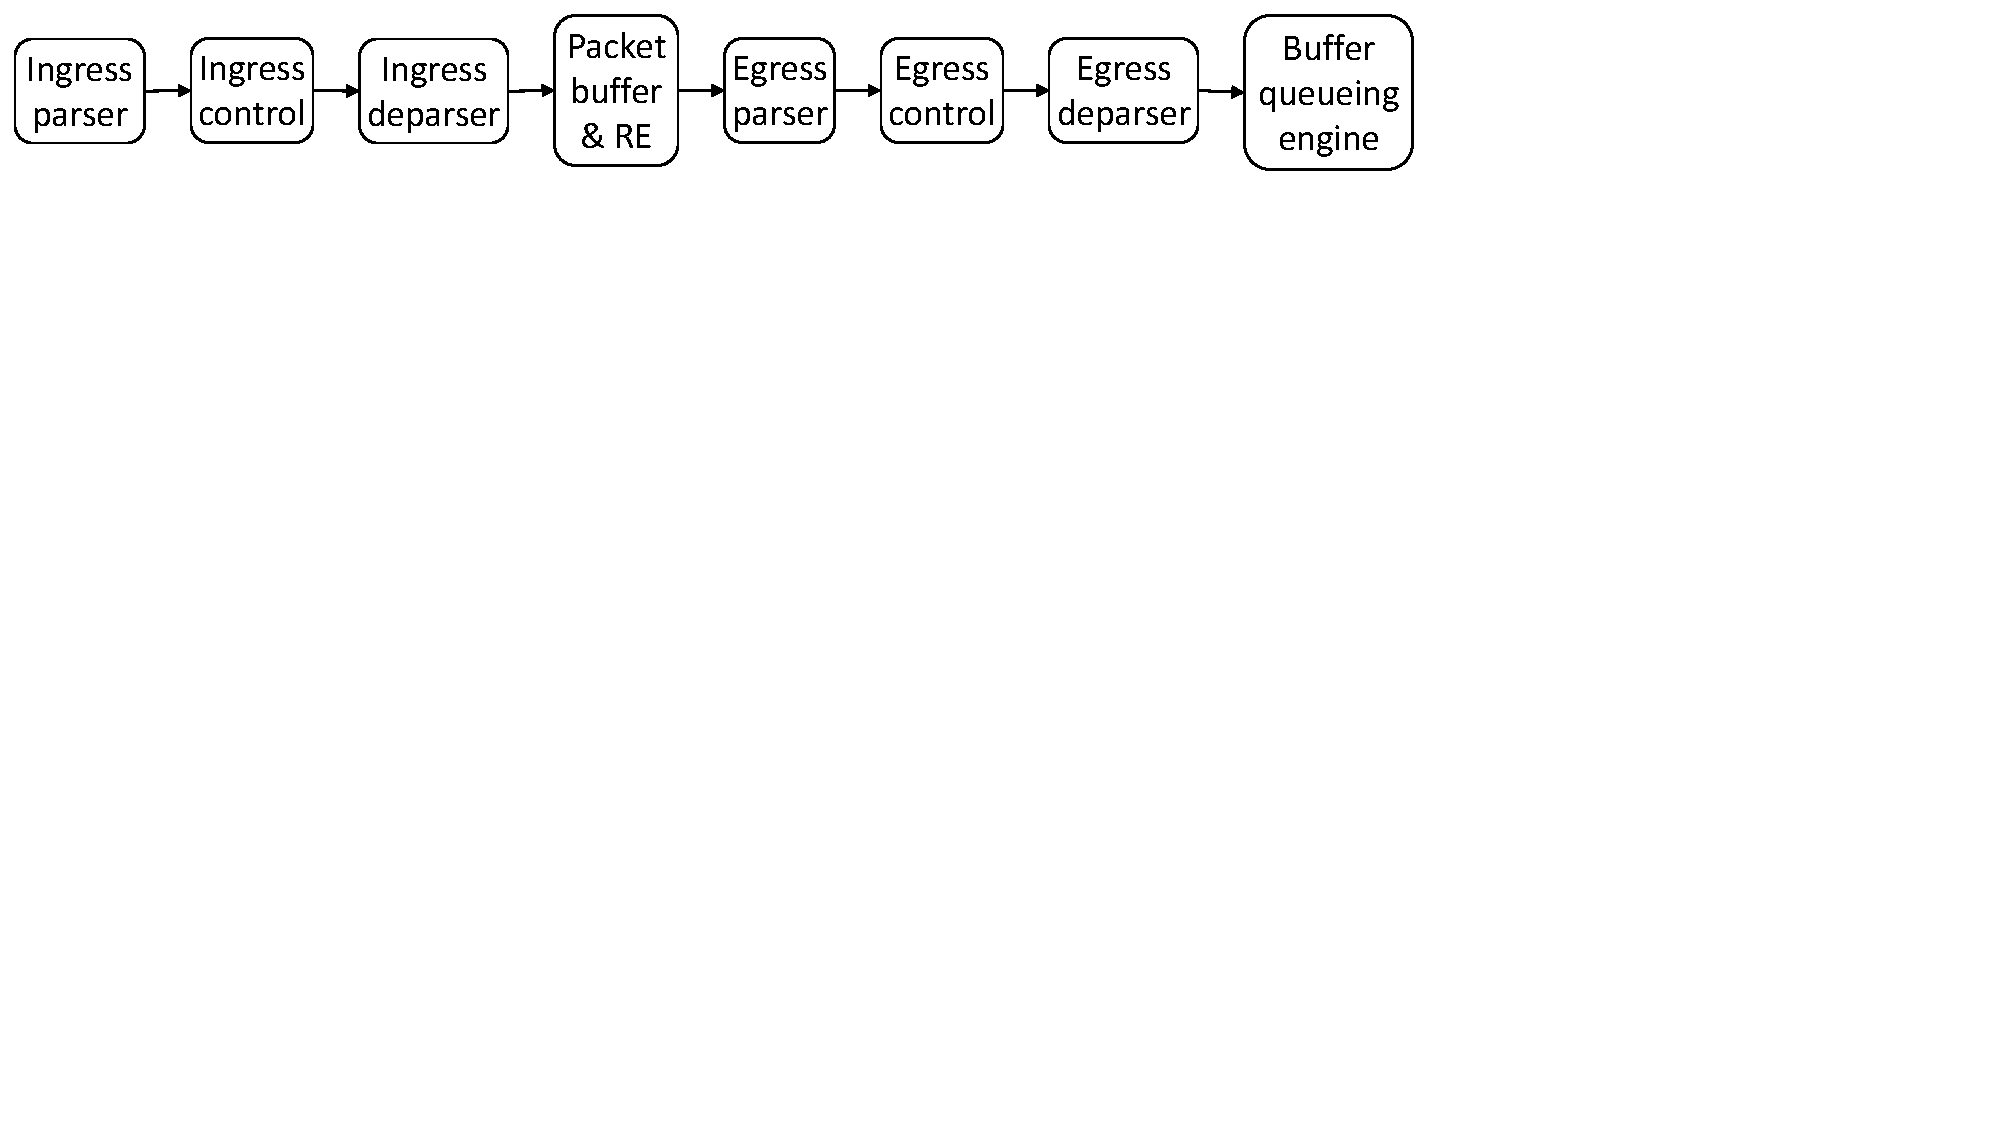
\includegraphics[trim=7 450 281 0, clip,scale=0.36]{psa-pipeline.pdf}
        \caption{PSA Model}
        \label{subfig:psa-model}
    \end{subfigure}
    \begin{subfigure}[b]{\linewidth}
        \centering
        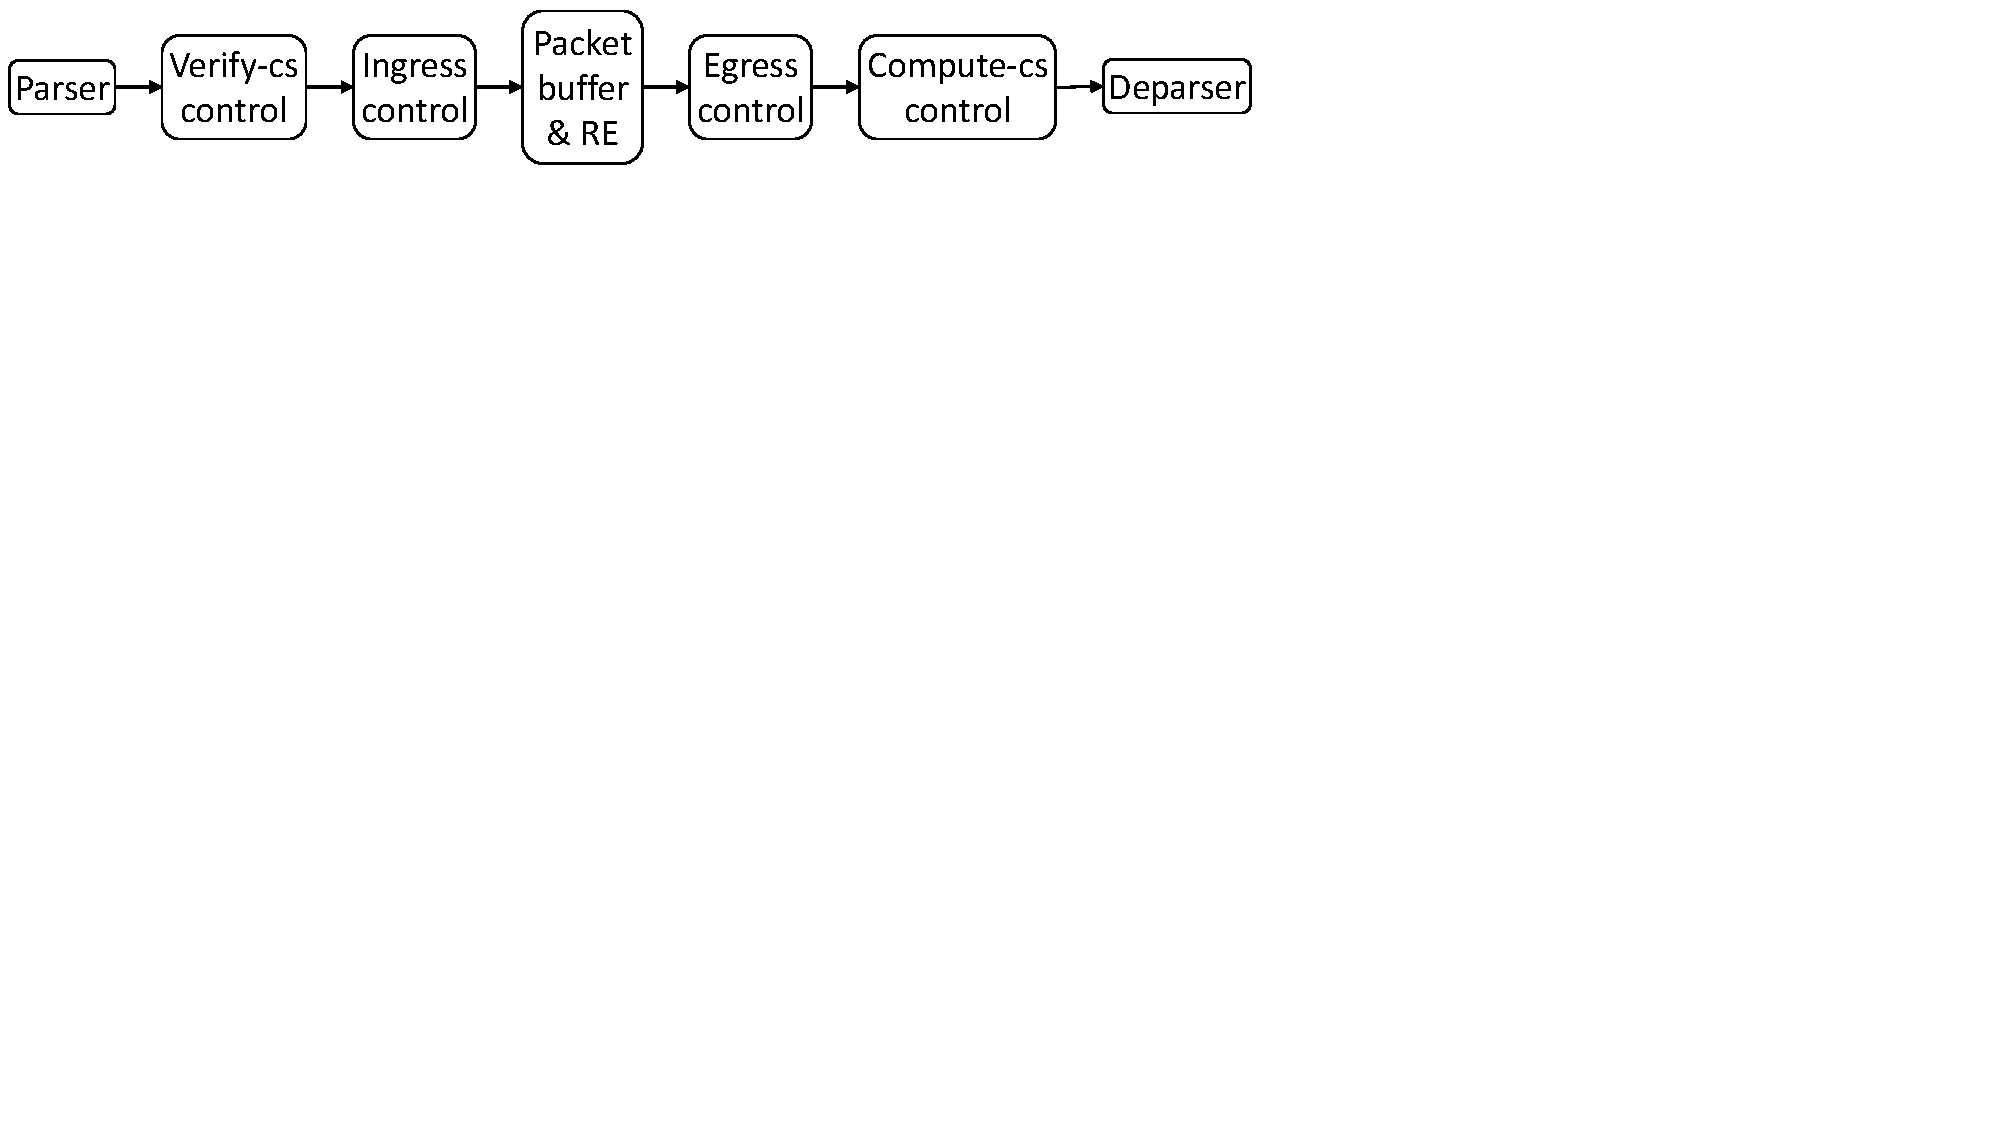
\includegraphics[trim=3 460 357 0, clip,scale=0.35]{v1model-pipeline.pdf}
        \caption{simple\_switch v1 Model}
        \label{subfig:v1model}
    \end{subfigure}
\caption{Real Target Architectures}
\label{fig:real-target-architectures}
\end{figure}



Parser blocks are described using a sub-language of P4, based on abstraction of Finite State Machine.
Control blocks are expressed using a sub-language modelling imperative control-flow.
Deparser are special control blocks that allows to use statements, to reassemble packets, that are not prohibited in other control blocks.
Therefore, packet processing logic of P4 programs are sectioned across programmable blocks with heterogeneous abstract machines (e.g., parsers, deparsers, control) and fixed-function blocks (Packet Buffer and Replication Engine).

Moreover, architectures models expose intrinsic metadata, target-specific actions and extern functions (e.g., resubmit, recirculate, clone) to replicate and/or program packet path and flow of data across the processing blocks.
<<For example, resubmit or recirculate calls are like event trigger.. effects happen after the block>>
In turn, adding different abstract-machine to program packet-path and data flow across the blocks and further increasing heterogeneity in the model of a data plane program.

Finally, the existing architecture models expose target-specific constraints.
E.g., output port can not be changed in egress control block, scope of some intrinsic metadata bounded by particular programmable blocks, etc.,  
Programmers need implement execution logic conforming to constraints, architecture model and semantics of actions and extern functions of the target device.


% P4 programmers need to implement homogeneous blocks (e.g., ingress and egress control) satisfying different accessibility constraints on intrinsic metadata exposed by the architecture. 
Due to absence of uniform abstract machine for a program and presence of constraints specific to programmable blocks, composition of data plane program modules is extremely difficult, even for the same target. 
Also, existing compilers and architecture specifications do not provide simplified and common abstractions for packet processing blocks in data plane to facilitate target agnostic reuse of data plane programs.


First, we simplify abstract machine for P4 data plane programs by reducing code fragmentation and programmable blocks.
Second, we abstract out fixed-function blocks by deriving logical constructs.
Third, we develop compiler mechanisms to have uniform abstract-machine for programmable blocks.
Finally, we translate our unified abstract machine and logical constructs into real target-specific heterogeneous packet-processing blocks, features and constraints.

In section~\ref{lbl:micros-switch-architecture-model}, we explain the design of Micro Switch Architecture for a logical target that reduces number of programmable blocks and introduces logical constructs to minimize heterogeneity in abstract model of a program.

\subsection{Micros Switch Architecture Model}
\label{lbl:micros-switch-architecture-model}


\begin{figure}
%  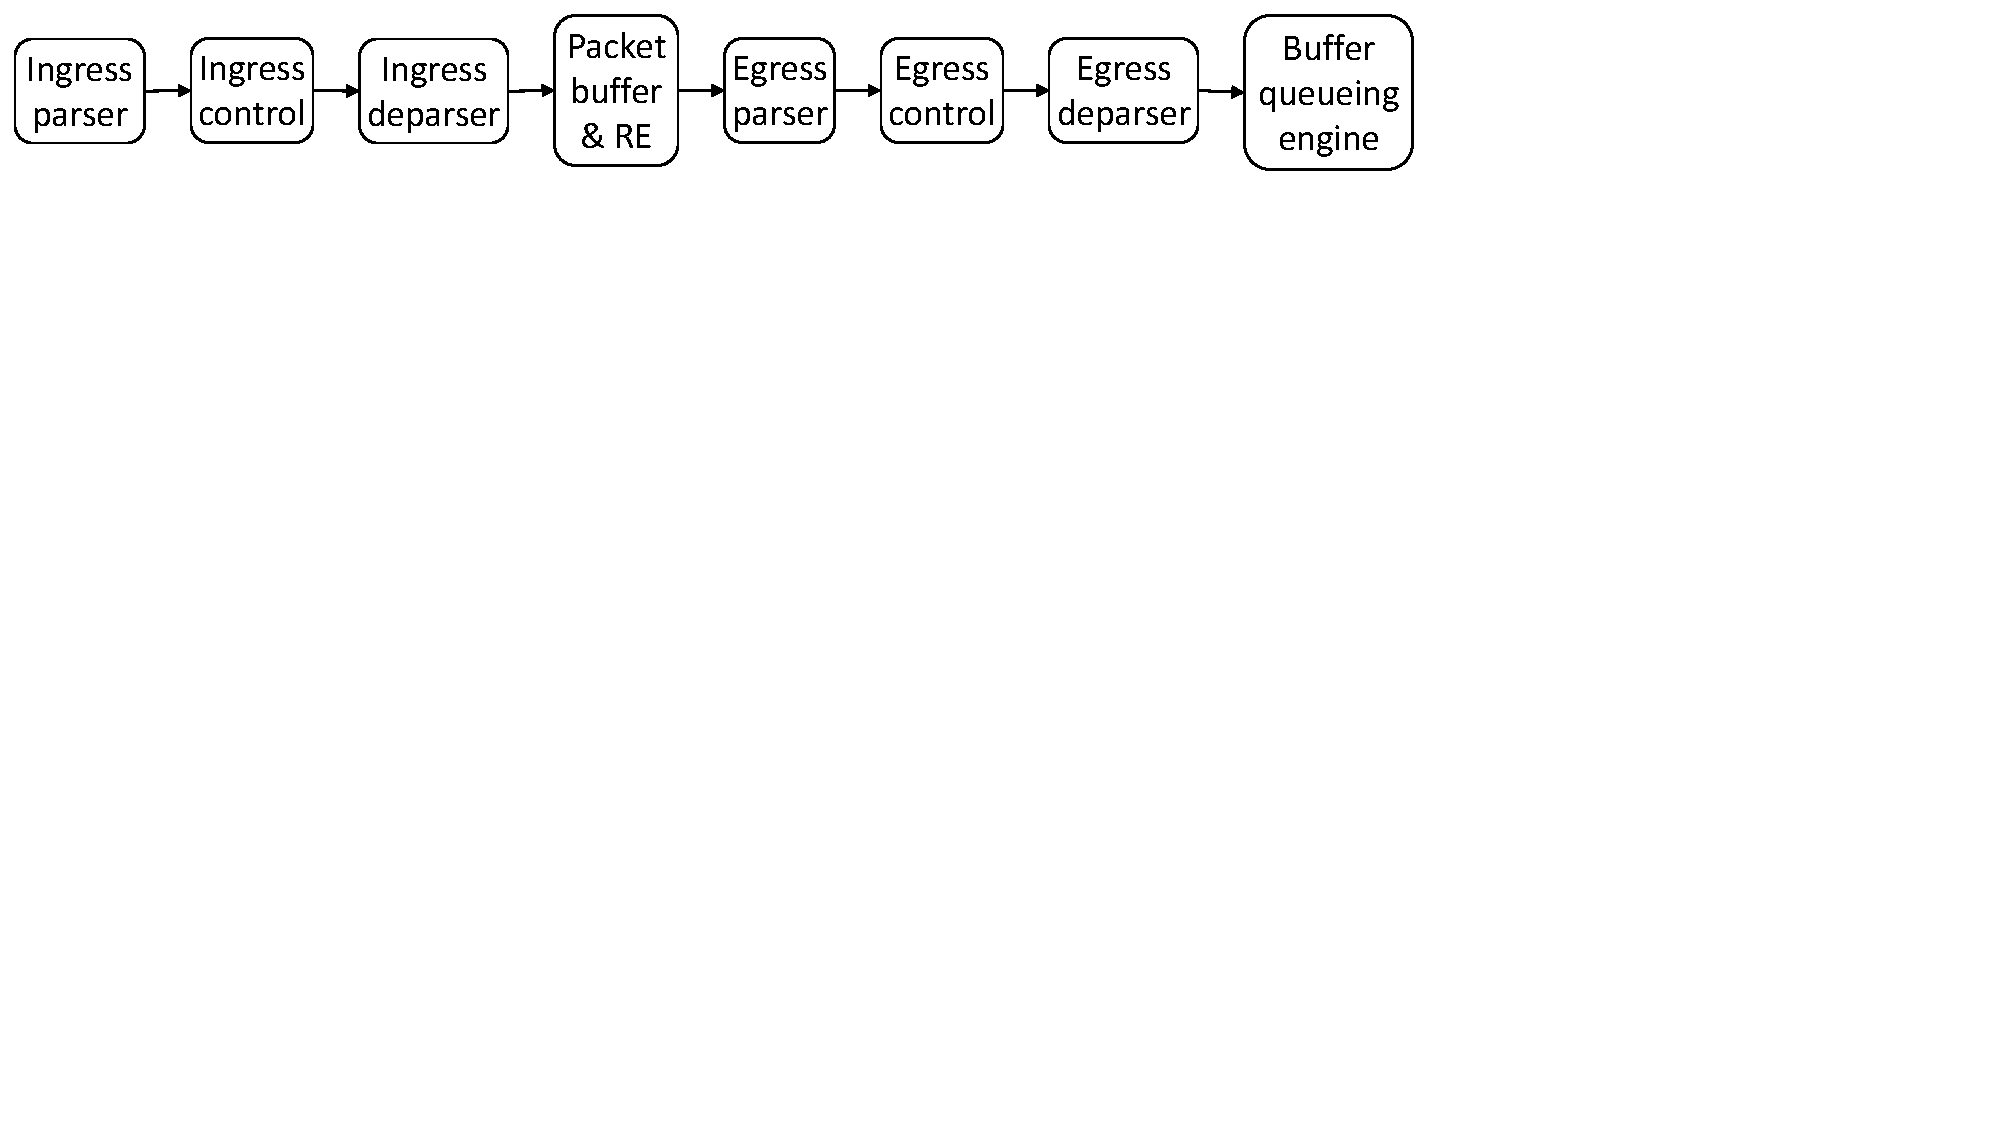
\includegraphics[trim=3 459 281 0, clip,scale=0.35]{psa-pipeline.pdf}
%  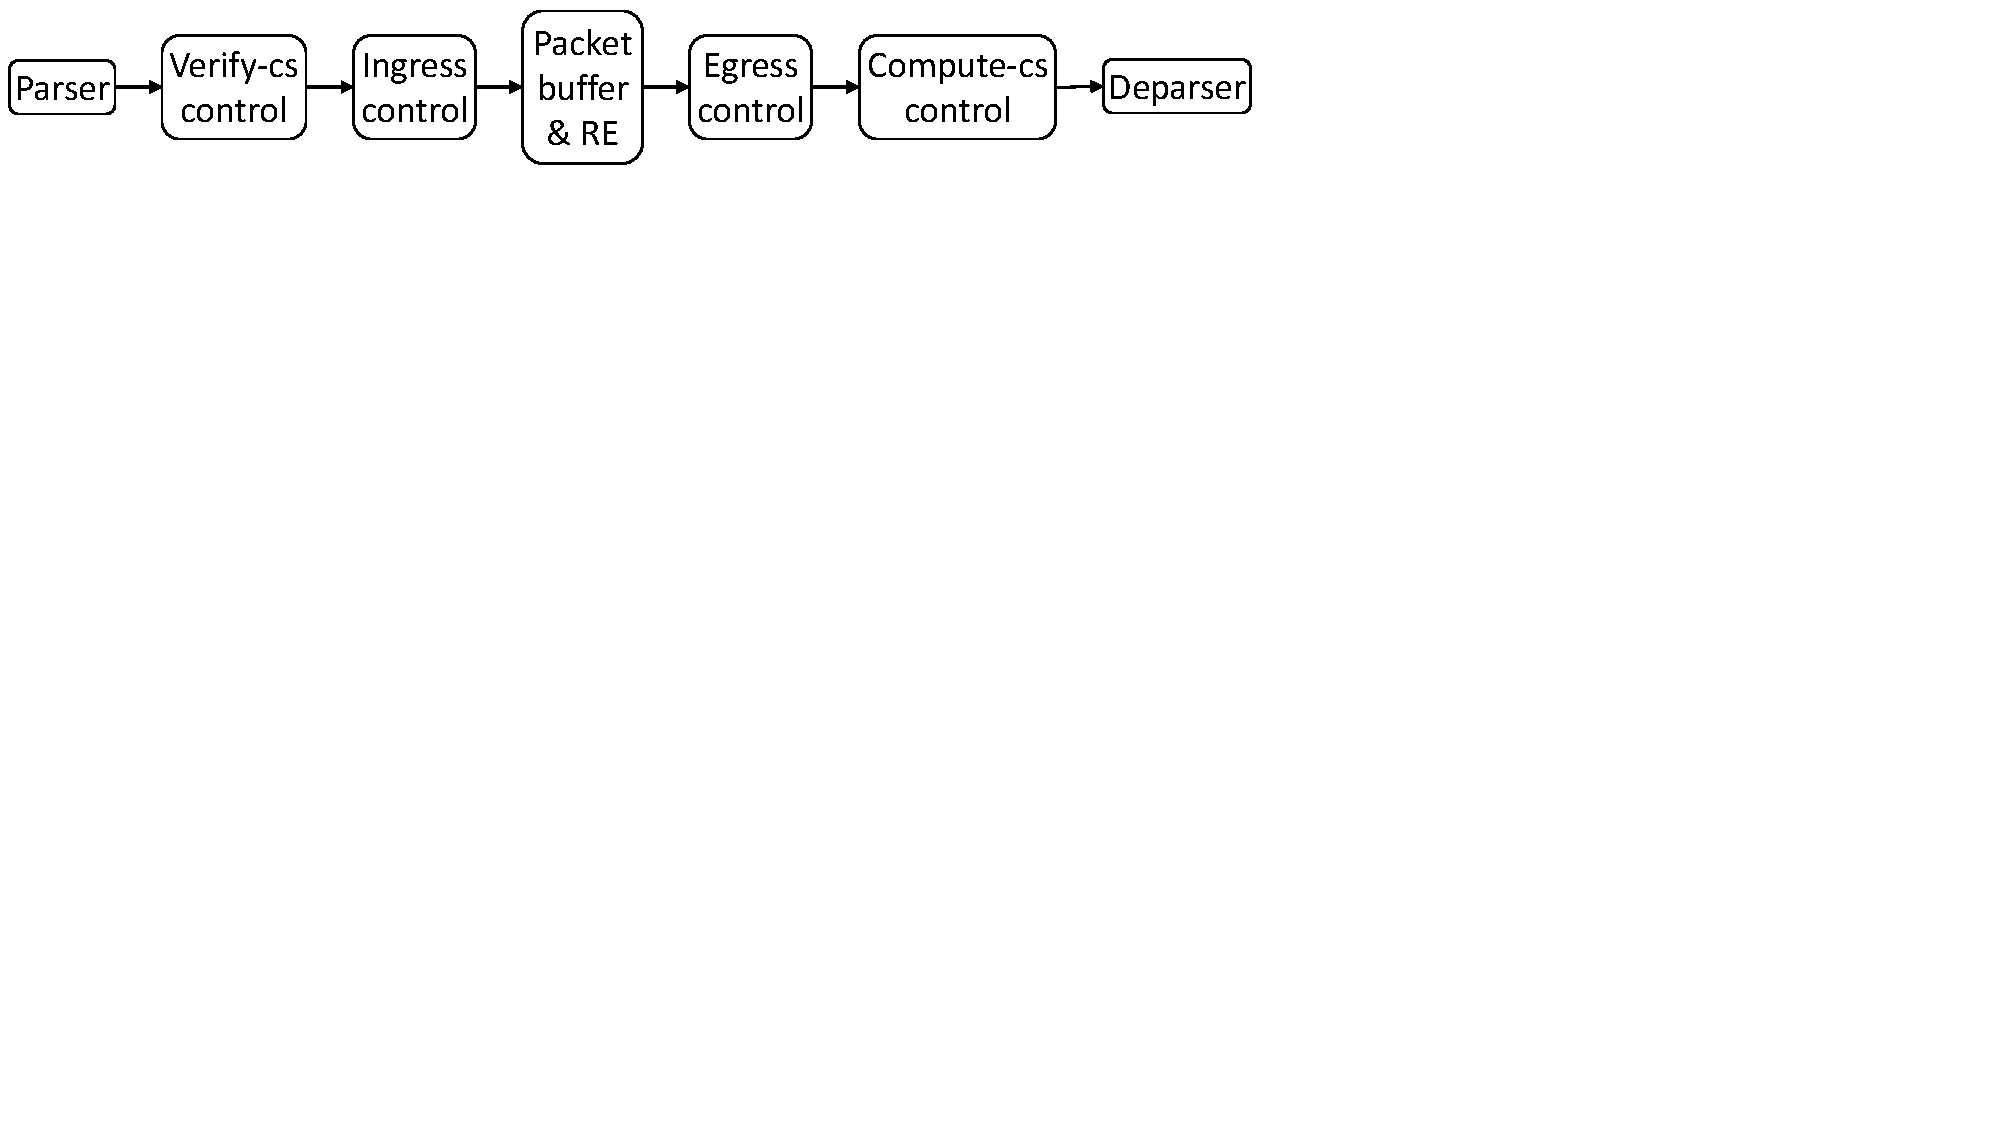
\includegraphics[trim=3 460 357 0, clip,scale=0.35]{v1model-pipeline.pdf}
%  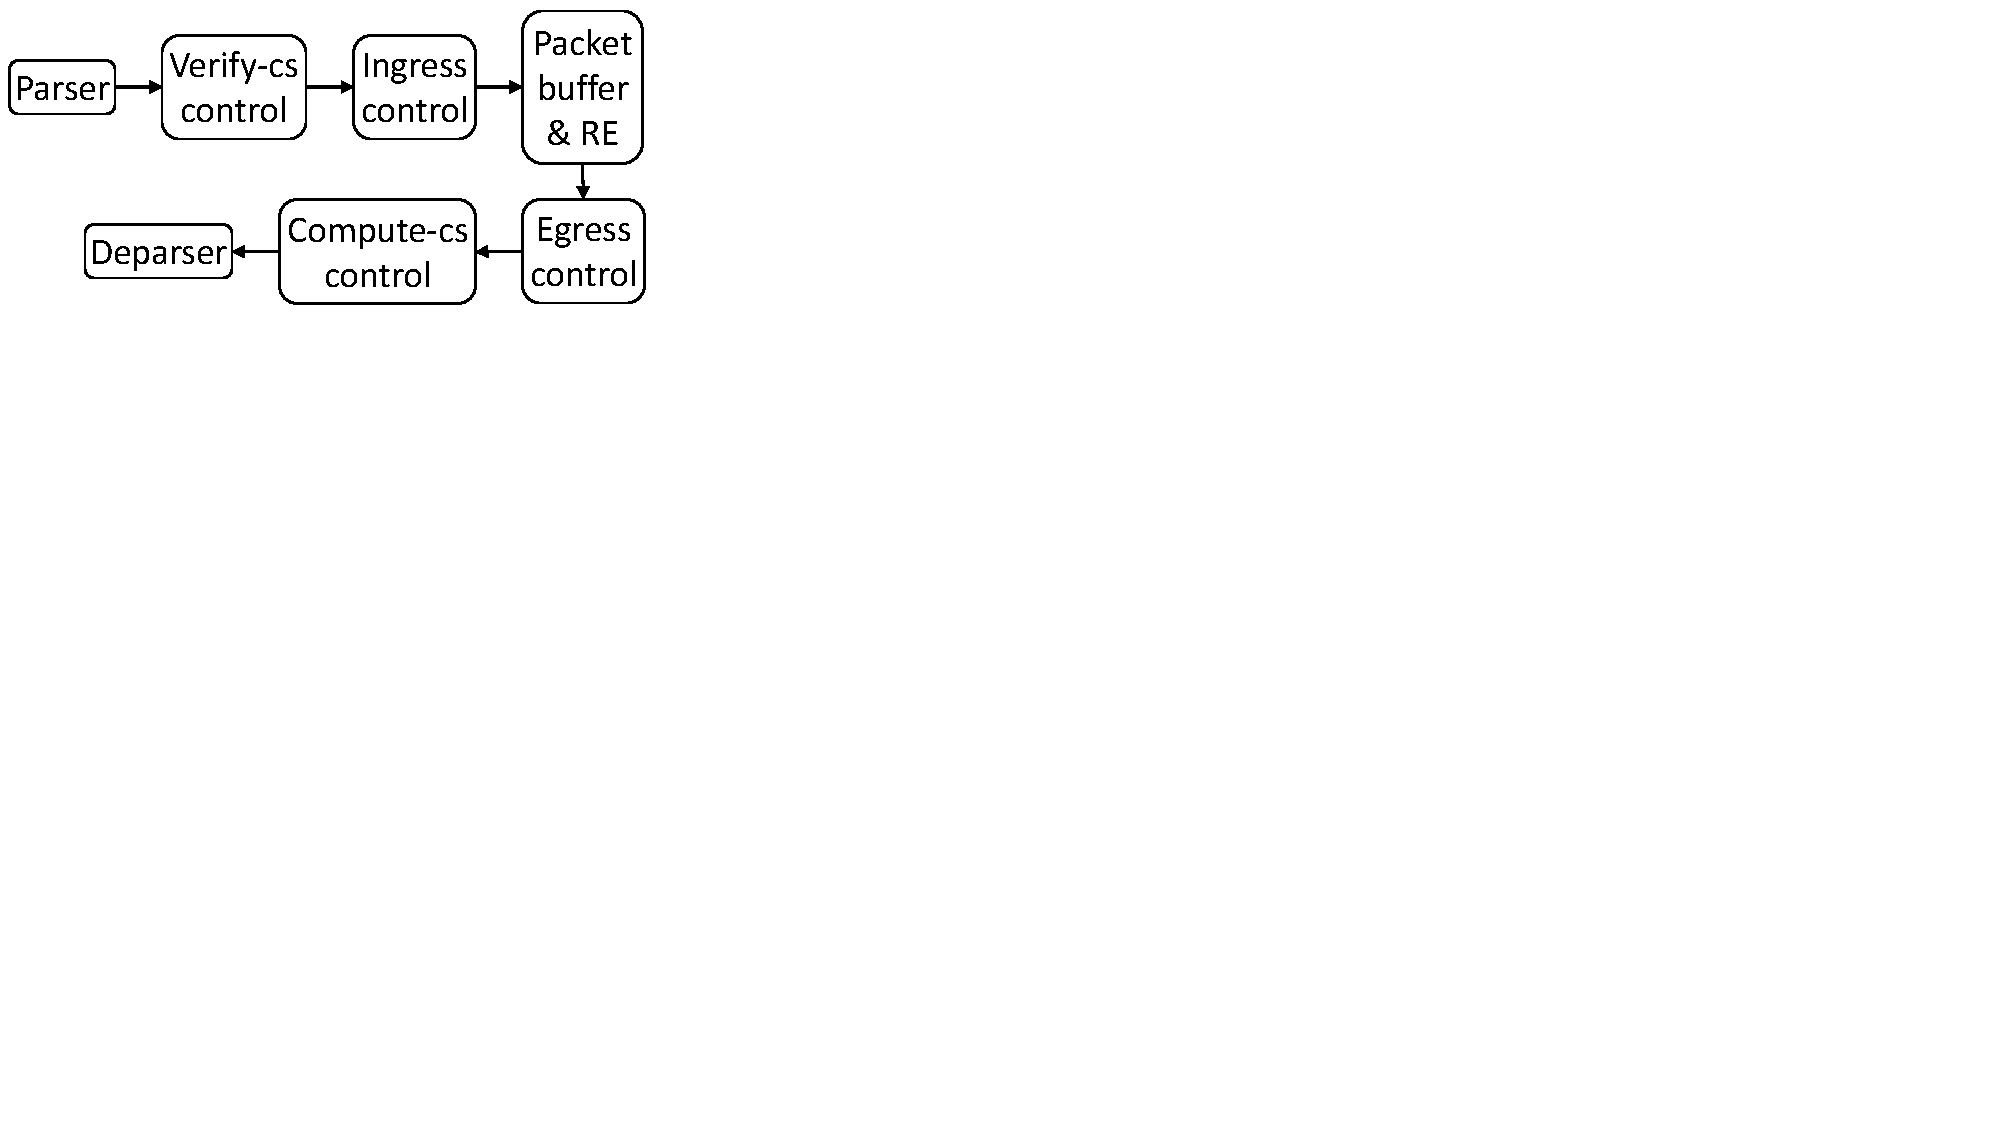
\includegraphics[trim=0 390 650 0, clip,scale=0.5]{v1model-pipeline-wrap.pdf}
%  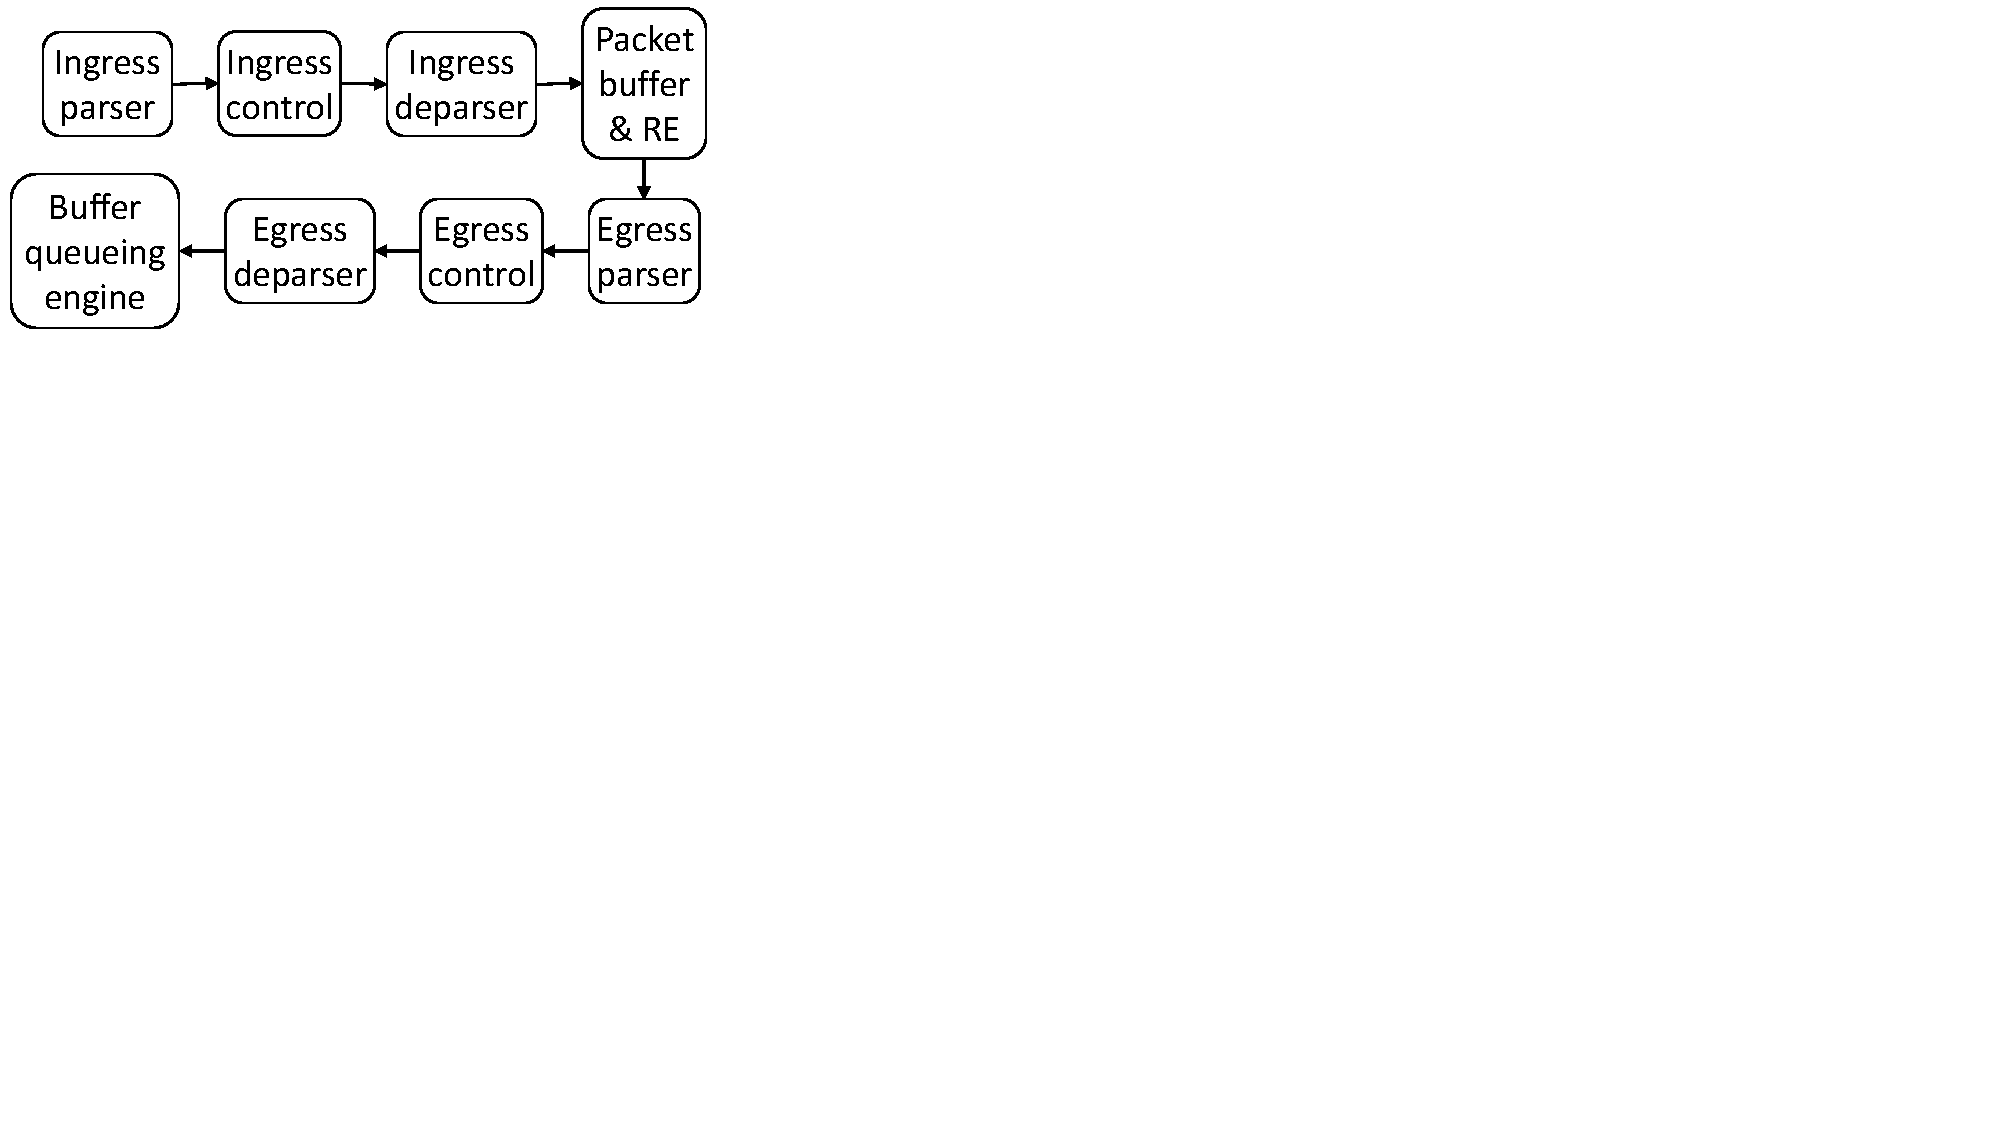
\includegraphics[trim=0 380 620 0, clip,scale=0.5]{psa-pipeline-wrap.pdf}
%  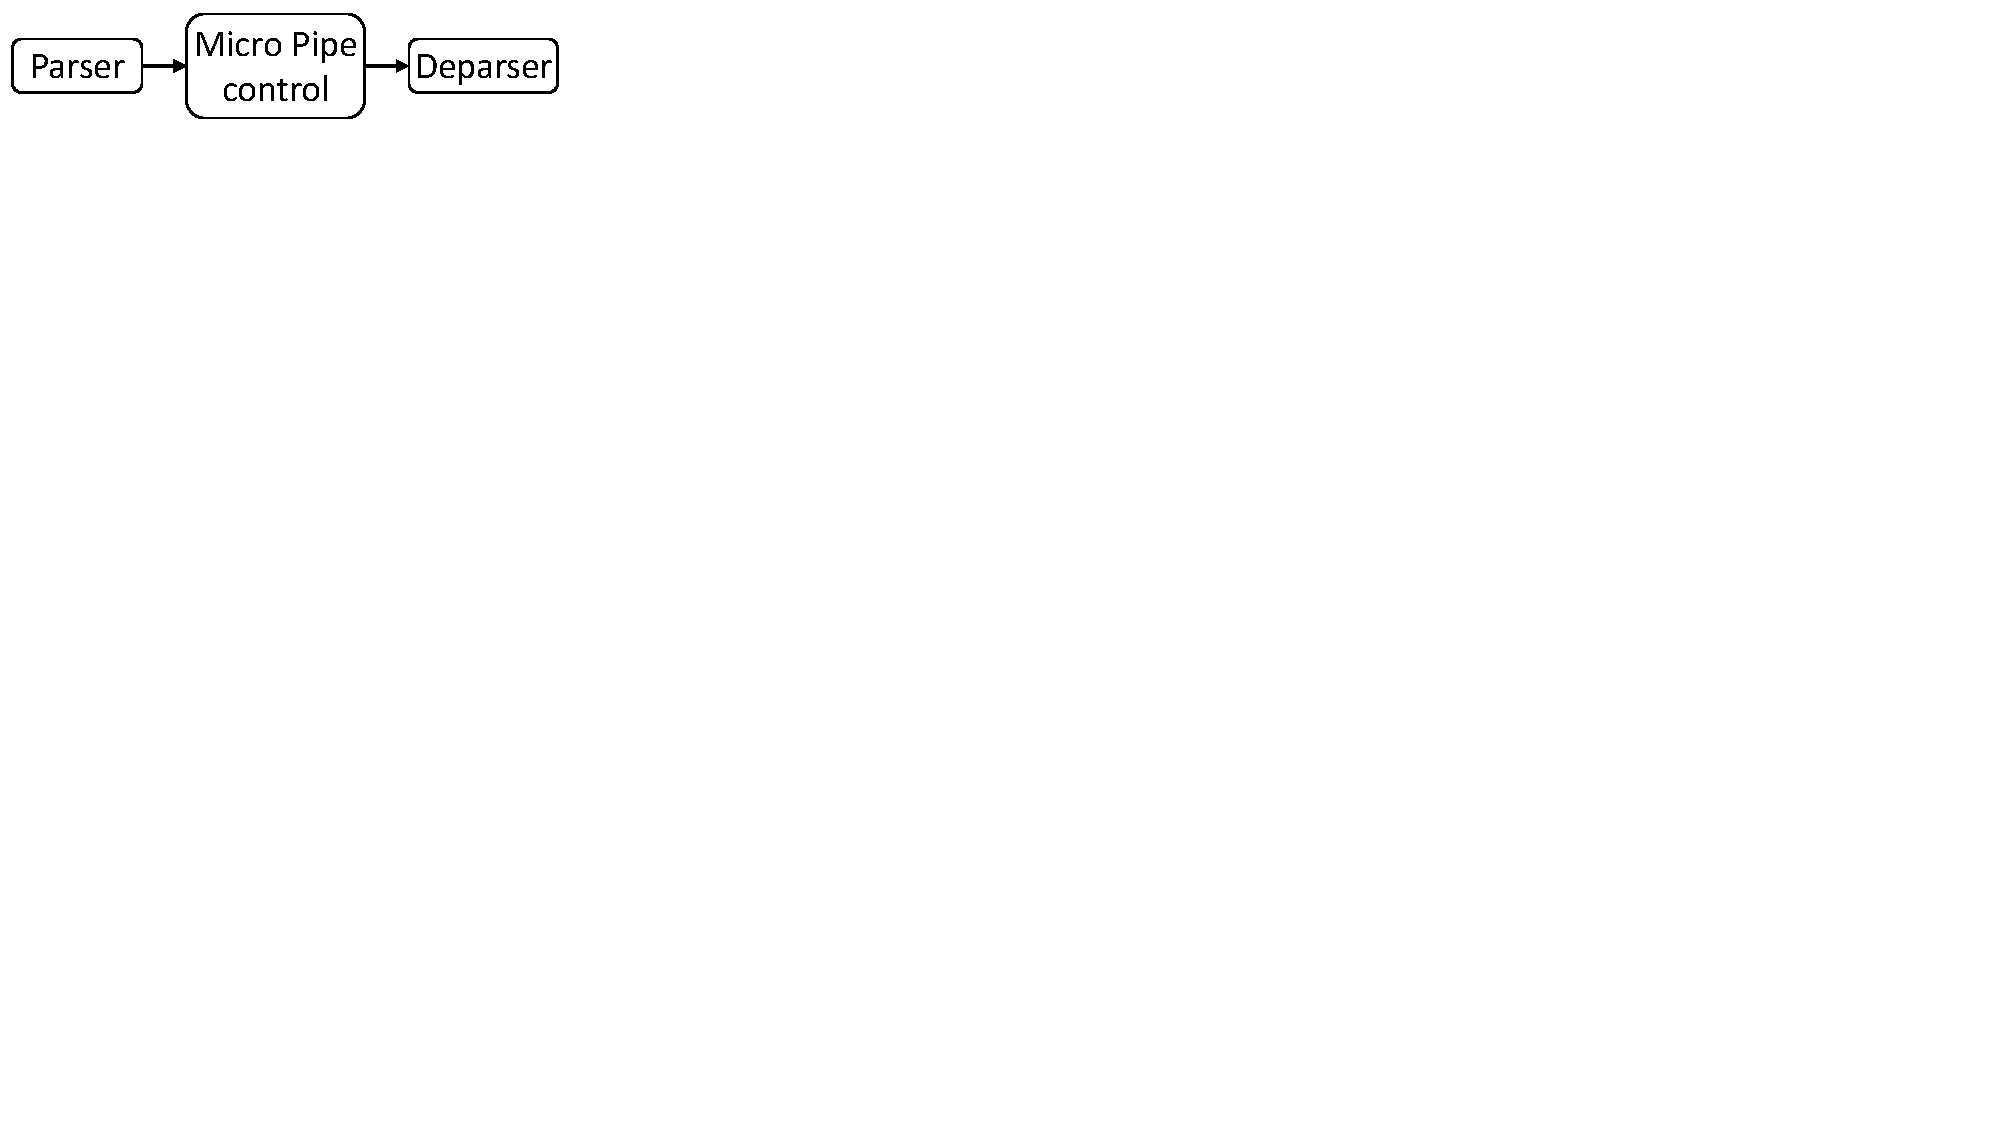
\includegraphics[trim=0 482 692 0, clip,scale=0.7]{msa-pipeline.pdf}
%  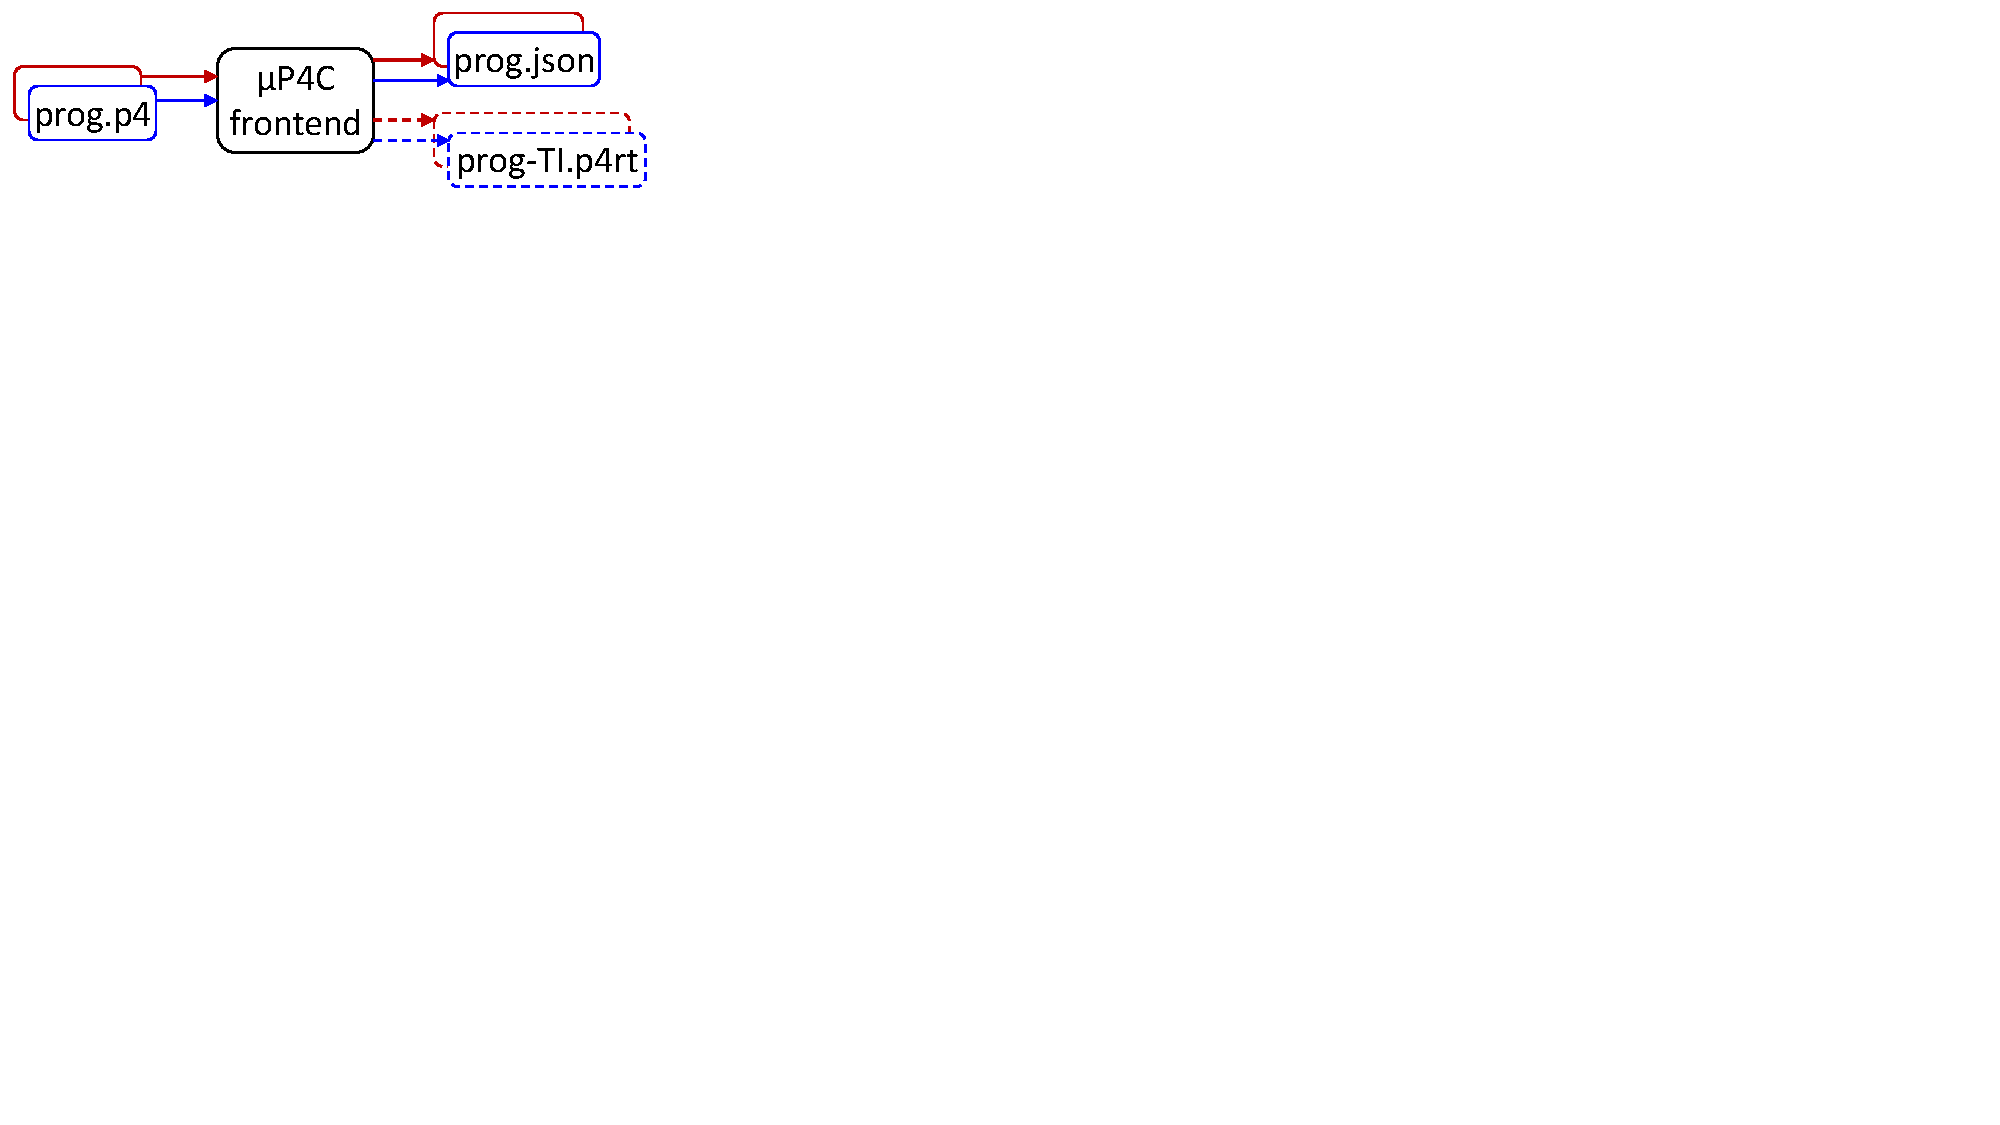
\includegraphics[trim=0 450 645 0, clip,scale=0.6]{mp4c-frontend.pdf}
%  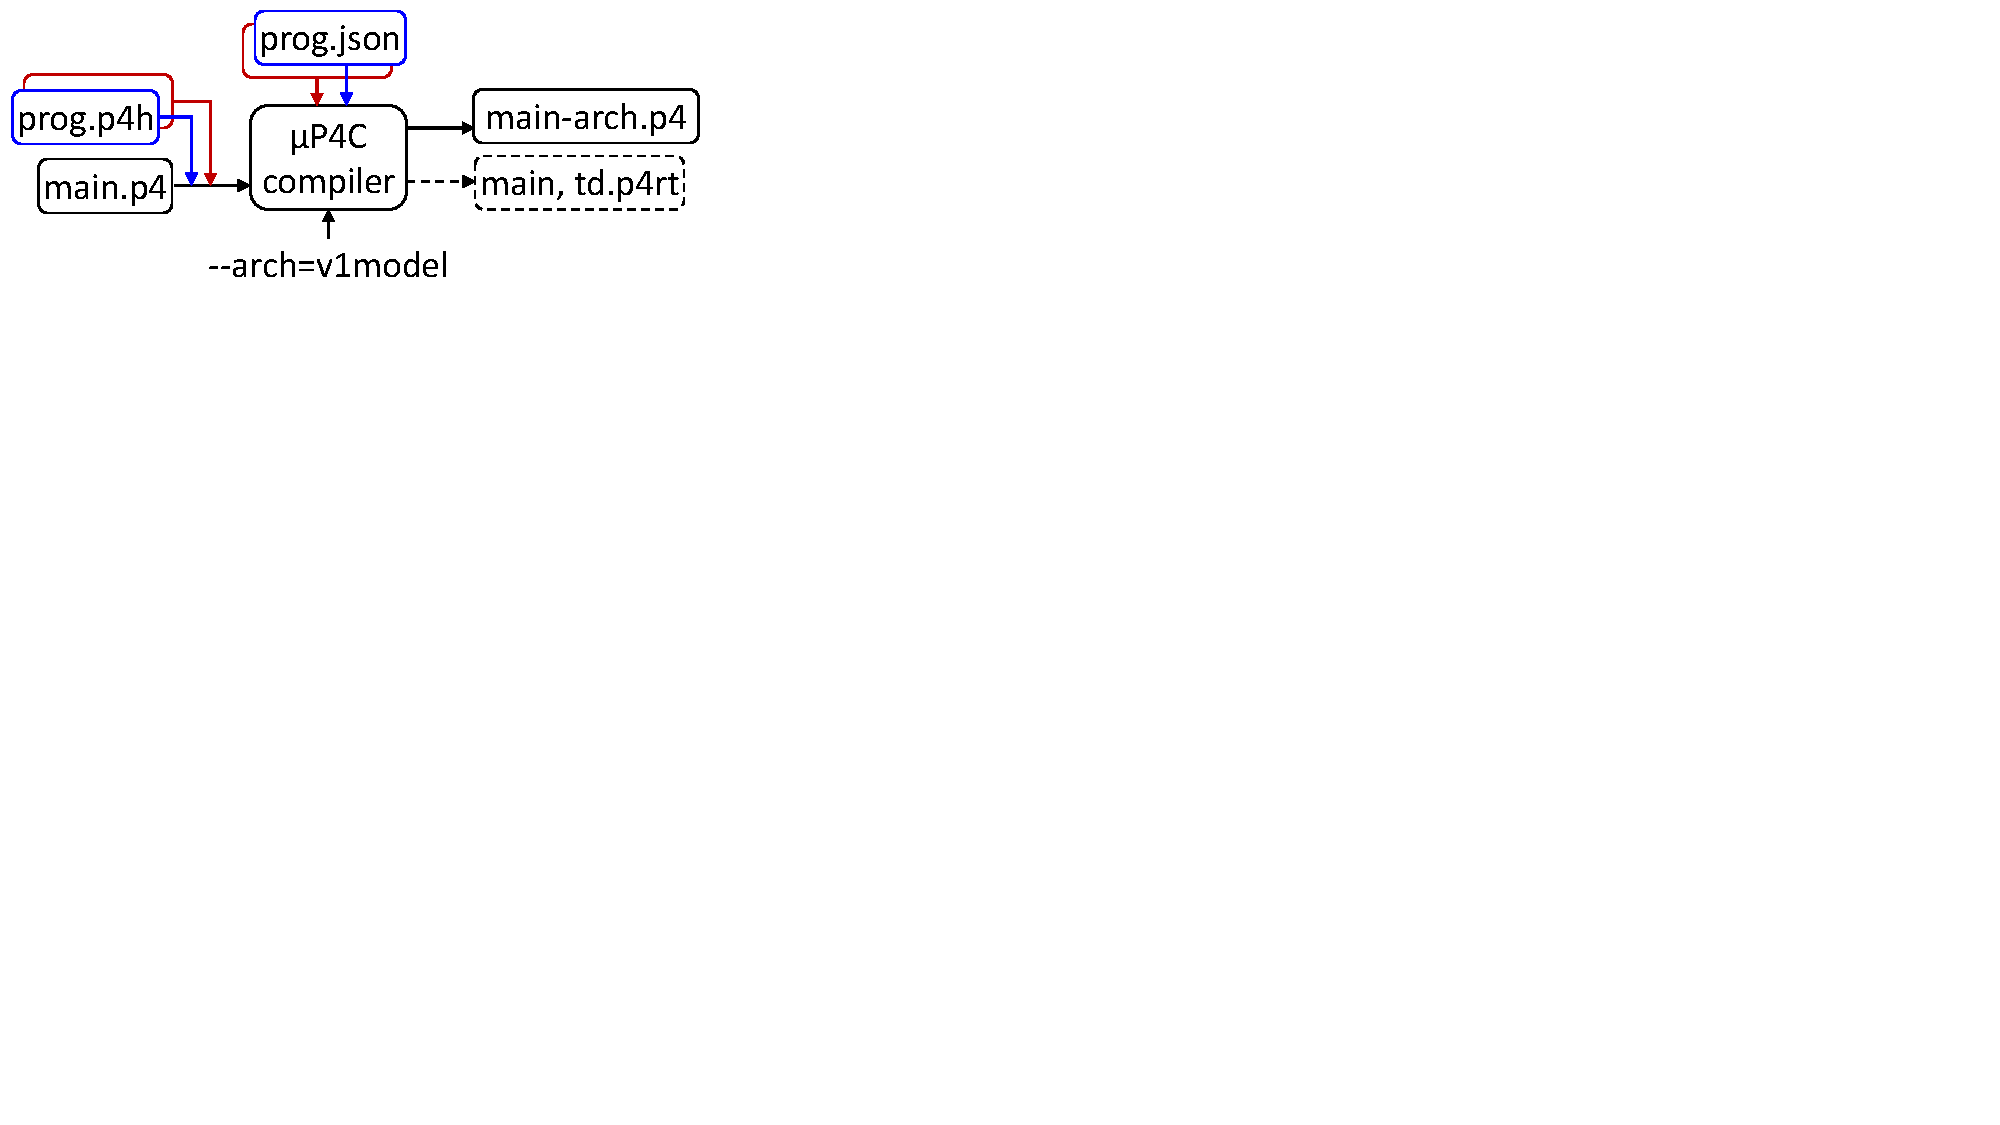
\includegraphics[trim=0 405 623 0, clip,scale=0.7]{mp4c-compiler}
%  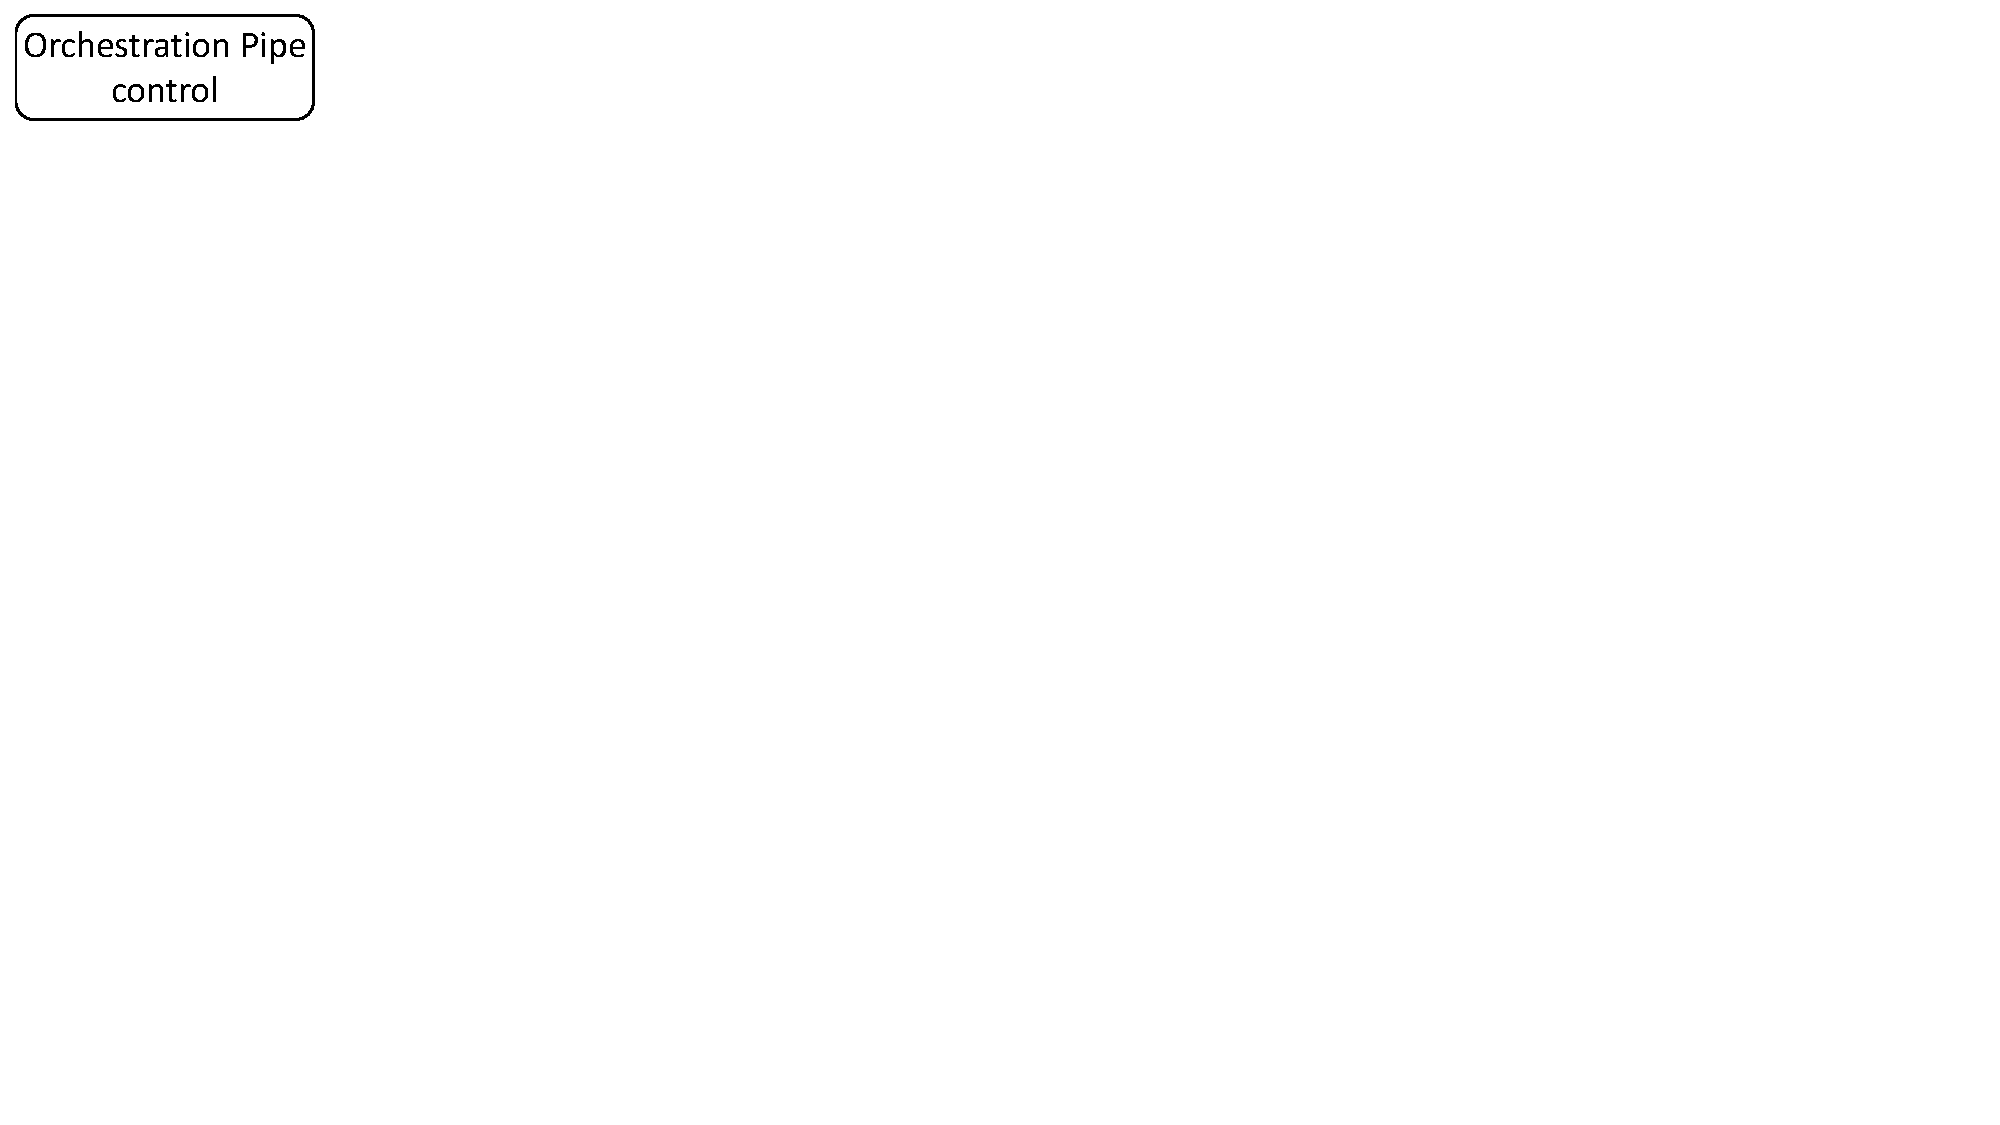
\includegraphics[trim=0 480 805 0,clip,scale=0.5]{micro-orchestration-pipeline}
\end{figure}

\subsubsection{Processing Blocks}
MSA provides two types of P4 packages interfaces, MicroSwitch and OrchestrationSwitch.
Programmers can provides implementations of 
has three programmable blocks, parser, pipe control and deparser control. 



\section{Compiler}

\subsection{Parser/Deparser Transformation}
converting parser and deparser into control blocks

\subsection{Architecture Translation}
Explain constraint.. take an example and show split of control-flow graph



\section{implementation}

\section{Related Work}

All data and control plane and policy composition related work 
pyretic, covisor
p4bricks
\section{Conclusion}

%%
%% The acknowledgments section is defined using the "acks" environment
%% (and NOT an unnumbered section). This ensures the proper
%% identification of the section in the article metadata, and the
%% consistent spelling of the heading.
\begin{acks}
...
\end{acks}

%%
%% The next two lines define the bibliography style to be used, and
%% the bibliography file.
\bibliographystyle{ACM-Reference-Format}
\bibliography{main}

%%
%% If your work has an appendix, this is the place to put it.
%% \appendix



\end{document}
\endinput
%%
%% End of file `sample-sigconf.tex'.
